\subsection{Программная реализация Диффи-Хеллмана}

\subsubsection{Структура класса и зависимости}
Реализация протокола инкапсулирована в класс `DiffieHellman`, который, аналогично `RSA`, наследуется от абстрактного базового класса `Protocol`. Это обеспечивает унифицированный интерфейс для всех криптографических протоколов в системе. Для работы с большими числами, необходимыми для криптографической стойкости, используется библиотека `Boost.Multiprecision` с типом `BigInt`. Интеграция с пользовательским интерфейсом Qt обеспечивается за счет использования типа `QString` для текстовых данных.

\begin{nvimstyle}
#ifndef DIFFIE_HELLMAN_HPP
#define DIFFIE_HELLMAN_HPP

#include "protocol.hpp"

#include <boost/multiprecision/cpp_int.hpp>
#include <boost/random/mersenne_twister.hpp>

using BigInt = boost::multiprecision::cpp_int;

namespace CRYPTO
{
class DiffieHellman final : public Protocol
{
public:
	explicit DiffieHellman(unsigned int prime_bits = 512);
	void init() override;
\end{nvimstyle}

\begin{nvimstyle}
	QString encrypt(const QString& plaintext) override;
	QString decrypt(const QString& ciphertext) override;

	void generateSharedSecret();

	BigInt getPrime();
	BigInt getPublicKey() const;

	void setOtherPartyPublicKey(const BigInt& key);
	void setOtherPartyPrime(const BigInt& prime);

private:
	void generateParameters();
	void generateKeys();
    
	BigInt generatePrime(unsigned int bits, boost::random::mt19937& rng);

private:
	// --- Параметры и ключи Диффи-Хеллмана ---
	unsigned int m_prime_bits;

	// Публичные параметры, общие для обеих сторон
	BigInt m_p; // Простое число-модуль `p`
	BigInt m_g; // Первообразный корень (генератор) `g`

	// Ключи этого участника
	BigInt m_private_key; // Закрытый ключ (секретное число `a` или `b`)
	BigInt m_public_key;  // Открытый ключ (A = g^a mod p или B = g^b mod p)

	// Данные, полученные от другого участника
	BigInt m_other_party_public_key; // Открытый ключ другого участника (A или B)

	// Финальный результат
	BigInt m_shared_secret; // Общий секретный ключ `s = (B^a) mod p = (A^b) mod p`
};

} // namespace CRYPTO

#endif // DIFFIE_HELLMAN_HPP
\end{nvimstyle}

\subsubsection{Инициализация и генерация ключей}
В отличие от RSA, где одна сторона генерирует пару ключей, в протоколе DH каждый участник (назовем их Алиса и Боб) выполняет свой собственный процесс генерации. Этот процесс реализован в методе `init()`, который вызывает внутренний метод `generateParametersAndKeys()`.

\begin{enumerate}
    \item \textbf{Согласование публичных параметров.} На первом этапе обе стороны должны согласовать два числа: большое простое число $p$ (модуль) и целое число $g$ (генератор или первообразный корень по модулю $p$). В данной реализации каждый участник генерирует свое простое число $p$ с помощью вспомогательного метода `generatePrime()`, который использует тест Миллера-Рабина для проверки на простоту. Для симуляции предполагается, что участники "договариваются" об использовании одного из этих наборов параметров (на практике параметры $p$ и $g$ часто стандартизированы и общеизвестны). В качестве генератора $g$ для простоты используется константное значение $5$.

    \item \textbf{Генерация секретного ключа.} Каждый участник генерирует свой собственный секретный ключ — случайное целое число. Алиса генерирует число $a$, а Боб — $b$. Эти числа должны находиться в диапазоне $[2, p-2]$ и храниться в строжайшем секрете.
    
    \item \textbf{Вычисление открытого ключа.} Используя публичные параметры и свой секретный ключ, каждый участник вычисляет свой открытый ключ.
    \begin{itemize}
        \item Алиса вычисляет: $A = g^a \pmod{p}$
        \item Боб вычисляет: $B = g^b \pmod{p}$
    \end{itemize}
    Для выполнения модульного возведения в степень используется оптимизированная функция `boost::multiprecision::powm`.
\end{enumerate}

\begin{nvimstyle}
void DiffieHellman::generateParameters()
{
	boost::random::mt19937 rng(std::random_device {}());

	// Шаг 1: Генерация большого простого числа p
	m_p = generatePrime(m_prime_bits, rng);

	// Шаг 2: Выбор генератора g
	m_g = 5;
}

void DiffieHellman::generateKeys()
{
	boost::random::mt19937 rng(std::random_device {}());

	// Шаг 3: Генерация закрытого ключа `a`
	boost::multiprecision::uniform_int_distribution<BigInt> dist(2, m_p - 2);
	m_private_key = dist(rng);

	// Шаг 4: Вычисление открытого ключа A = g^a mod p
	m_public_key = boost::multiprecision::powm(m_g, m_private_key, m_p);
}
\end{nvimstyle}

\subsubsection{Обмен ключами и вычисление общего секрета}
После генерации ключей участники обмениваются своими открытыми ключами ($A$ и $B$) по публичному каналу. Процесс обмена и последующего вычисления общего секрета управляется классом `DiffieHellmanExchanger`.

\begin{enumerate}
    \item \textbf{Обмен.} Алиса отправляет Бобу свой открытый ключ $A$, а Боб отправляет Алисе свой ключ $B$. В программной реализации это симулируется вызовом метода `setOtherPartyPublicKey()`.

    \item \textbf{Вычисление общего секрета.} Получив открытый ключ другой стороны, каждый участник может вычислить общий секретный ключ $s$. Важнейшим свойством протокола является то, что обе стороны получают одинаковый результат, выполняя вычисления независимо друг от друга.
    \begin{itemize}
        \item Алиса вычисляет: $s = B^a \pmod{p} = (g^b)^a \pmod{p}$
        \item Боб вычисляет: $s = A^b \pmod{p} = (g^a)^b \pmod{p}$
    \end{itemize}
    В результате $s = g^{ab} \pmod{p}$ становится их общим секретом. Злоумышленник, перехвативший $p, g, A, B$, не может легко вычислить $s$, так как для этого ему потребуется решить задачу дискретного логарифмирования (найти $a$ из $A$ или $b$ из $B$).
\end{enumerate}

\begin{nvimstyle}
void DiffieHellman::generateSharedSecret()
{
	if (m_other_party_public_key == 0)
	{
		throw std::runtime_error("Открытый ключ другого участника не установлен.");
	}

	// Вычисление общего секрета: s = (B^a) mod p
	m_shared_secret = boost::multiprecision::powm(m_other_party_public_key, m_private_key, m_p);
}
\end{nvimstyle}


\subsubsection{Использование общего секрета для шифрования}
Протокол Диффи-Хеллмана предназначен исключительно для обмена ключами и не является протоколом шифрования. Однако для демонстрации успешного установления общего секрета были реализованы методы `encrypt()` и `decrypt()`, которые используют полученный ключ $s$ для симметричного шифрования.

\begin{enumerate}
    \item \textbf{Преобразование данных.} Входная строка `QString` преобразуется в массив байтов `QByteArray` в кодировке UTF-8, а затем в большое целое число `BigInt`.
    
    \item \textbf{Операция шифрования/расшифрования.} В качестве симметричного шифра используется простая операция побитового исключающего "ИЛИ" (XOR) между числовым представлением сообщения и общим секретным ключом $s$.
    \begin{itemize}
        \item Шифрование: `ciphertext\_int = plaintext\_int XOR s`
        \item Расшифрование: `plaintext\_int = ciphertext\_int XOR s`
    \end{itemize}
    Так как операция XOR является обратимой, один и тот же метод фактически выполняет и шифрование, и расшифрование.

    \item \textbf{Формат передачи.} Для передачи зашифрованные данные преобразуются в шестнадцатеричную строку. При расшифровании выполняется обратное преобразование из шестнадцатеричной строки в `BigInt`.
\end{enumerate}

\subsection{Пример работы протокола Диффи-Хеллмана}
На рисунке ниже продемонстрирован интерфейс виджета, симулирующего работу протокола. После нажатия на кнопку "Выполнить обмен ключами (DH)" в логе отображается процесс установления общего секрета. Затем Алиса и Боб могут обмениваться зашифрованными сообщениями, подтверждая, что они обладают одним и тем же ключом.

\begin{figure}[htbp]
    \centering 
    \subfloat[Key exchange]{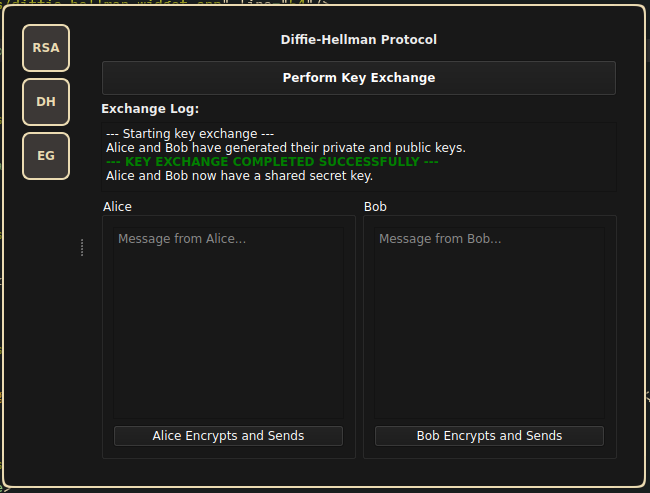
\includegraphics[width=0.48\textwidth]{res/png/04_dh_key_exchange.png}\label{fig:sub1}}
    \hfill
    \subfloat[Message exchange]{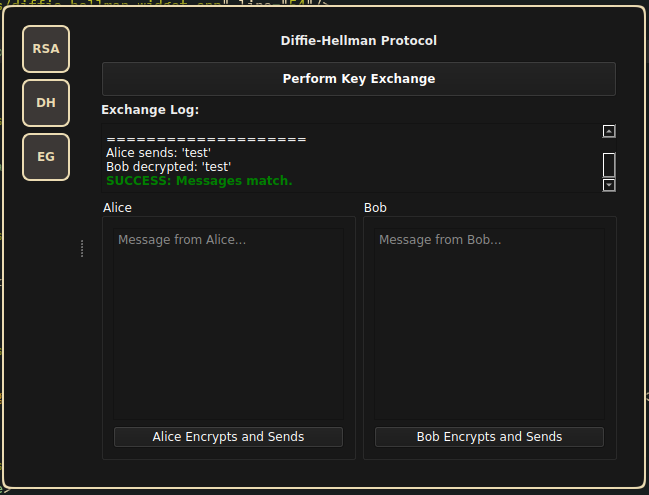
\includegraphics[width=0.48\textwidth]{res/png/05_dh_message_send.png}\label{fig:sub2}}
    \label{fig:side_by_side}
\end{figure}